% Chapter 4

\chapter{Time series anomaly detection in grid load issue} % Main chapter title

\label{Chapter4} % For referencing the chapter elsewhere, use \ref{Chapter1} 
\setlength{\parindent}{0pt}
%----------------------------------------------------------------------------------------

We will try to model and refine our predictions and detections on electronic grid load issues with the base of understanding existing models and characters of kinds of data set. There are two kinds of reasons to choose such a special problem to solve. One is that compared to other kinds of sequential data; grid load data is relatively stable and cyclic. This feature makes it more factorable to label or locate "anomaly period" so that our model could have more application beyond one certain dataset. On the other hand, all the datasets in Chapter3 we have tested are offered by university labs and commonly used in machine learning tasks. They were elaborative preprocessed already and might make significance in new model checking than application. 

\section{Data Description}
For grid load data, anomaly detection is useful but might be ignored by many analysts. Not only to deal with grid supply smarter, energy-saving, and could prevent fire caused by over-electricity load, but also, could be used into crime capture or financial evaluations(like loan limitations for factories), because nearly all the activities need electronic equipment and once we detect anomaly load in some subsection of the grid, i.e., distinct or state levels, might reflect some vital changes in producing or daily lives. 

We used GEFCom2014 (Electric load forecasting) as our mainly dataset to train our models, a probabilistic energy forecasting competition with four tracks on load, price, wind and solar forecasting, which attracted 581 participants from 61 countries. And we draw a basic trends plot for it, as Figure \ref{fig:gefc2014} shows.

% \begin{figure}[H]
%     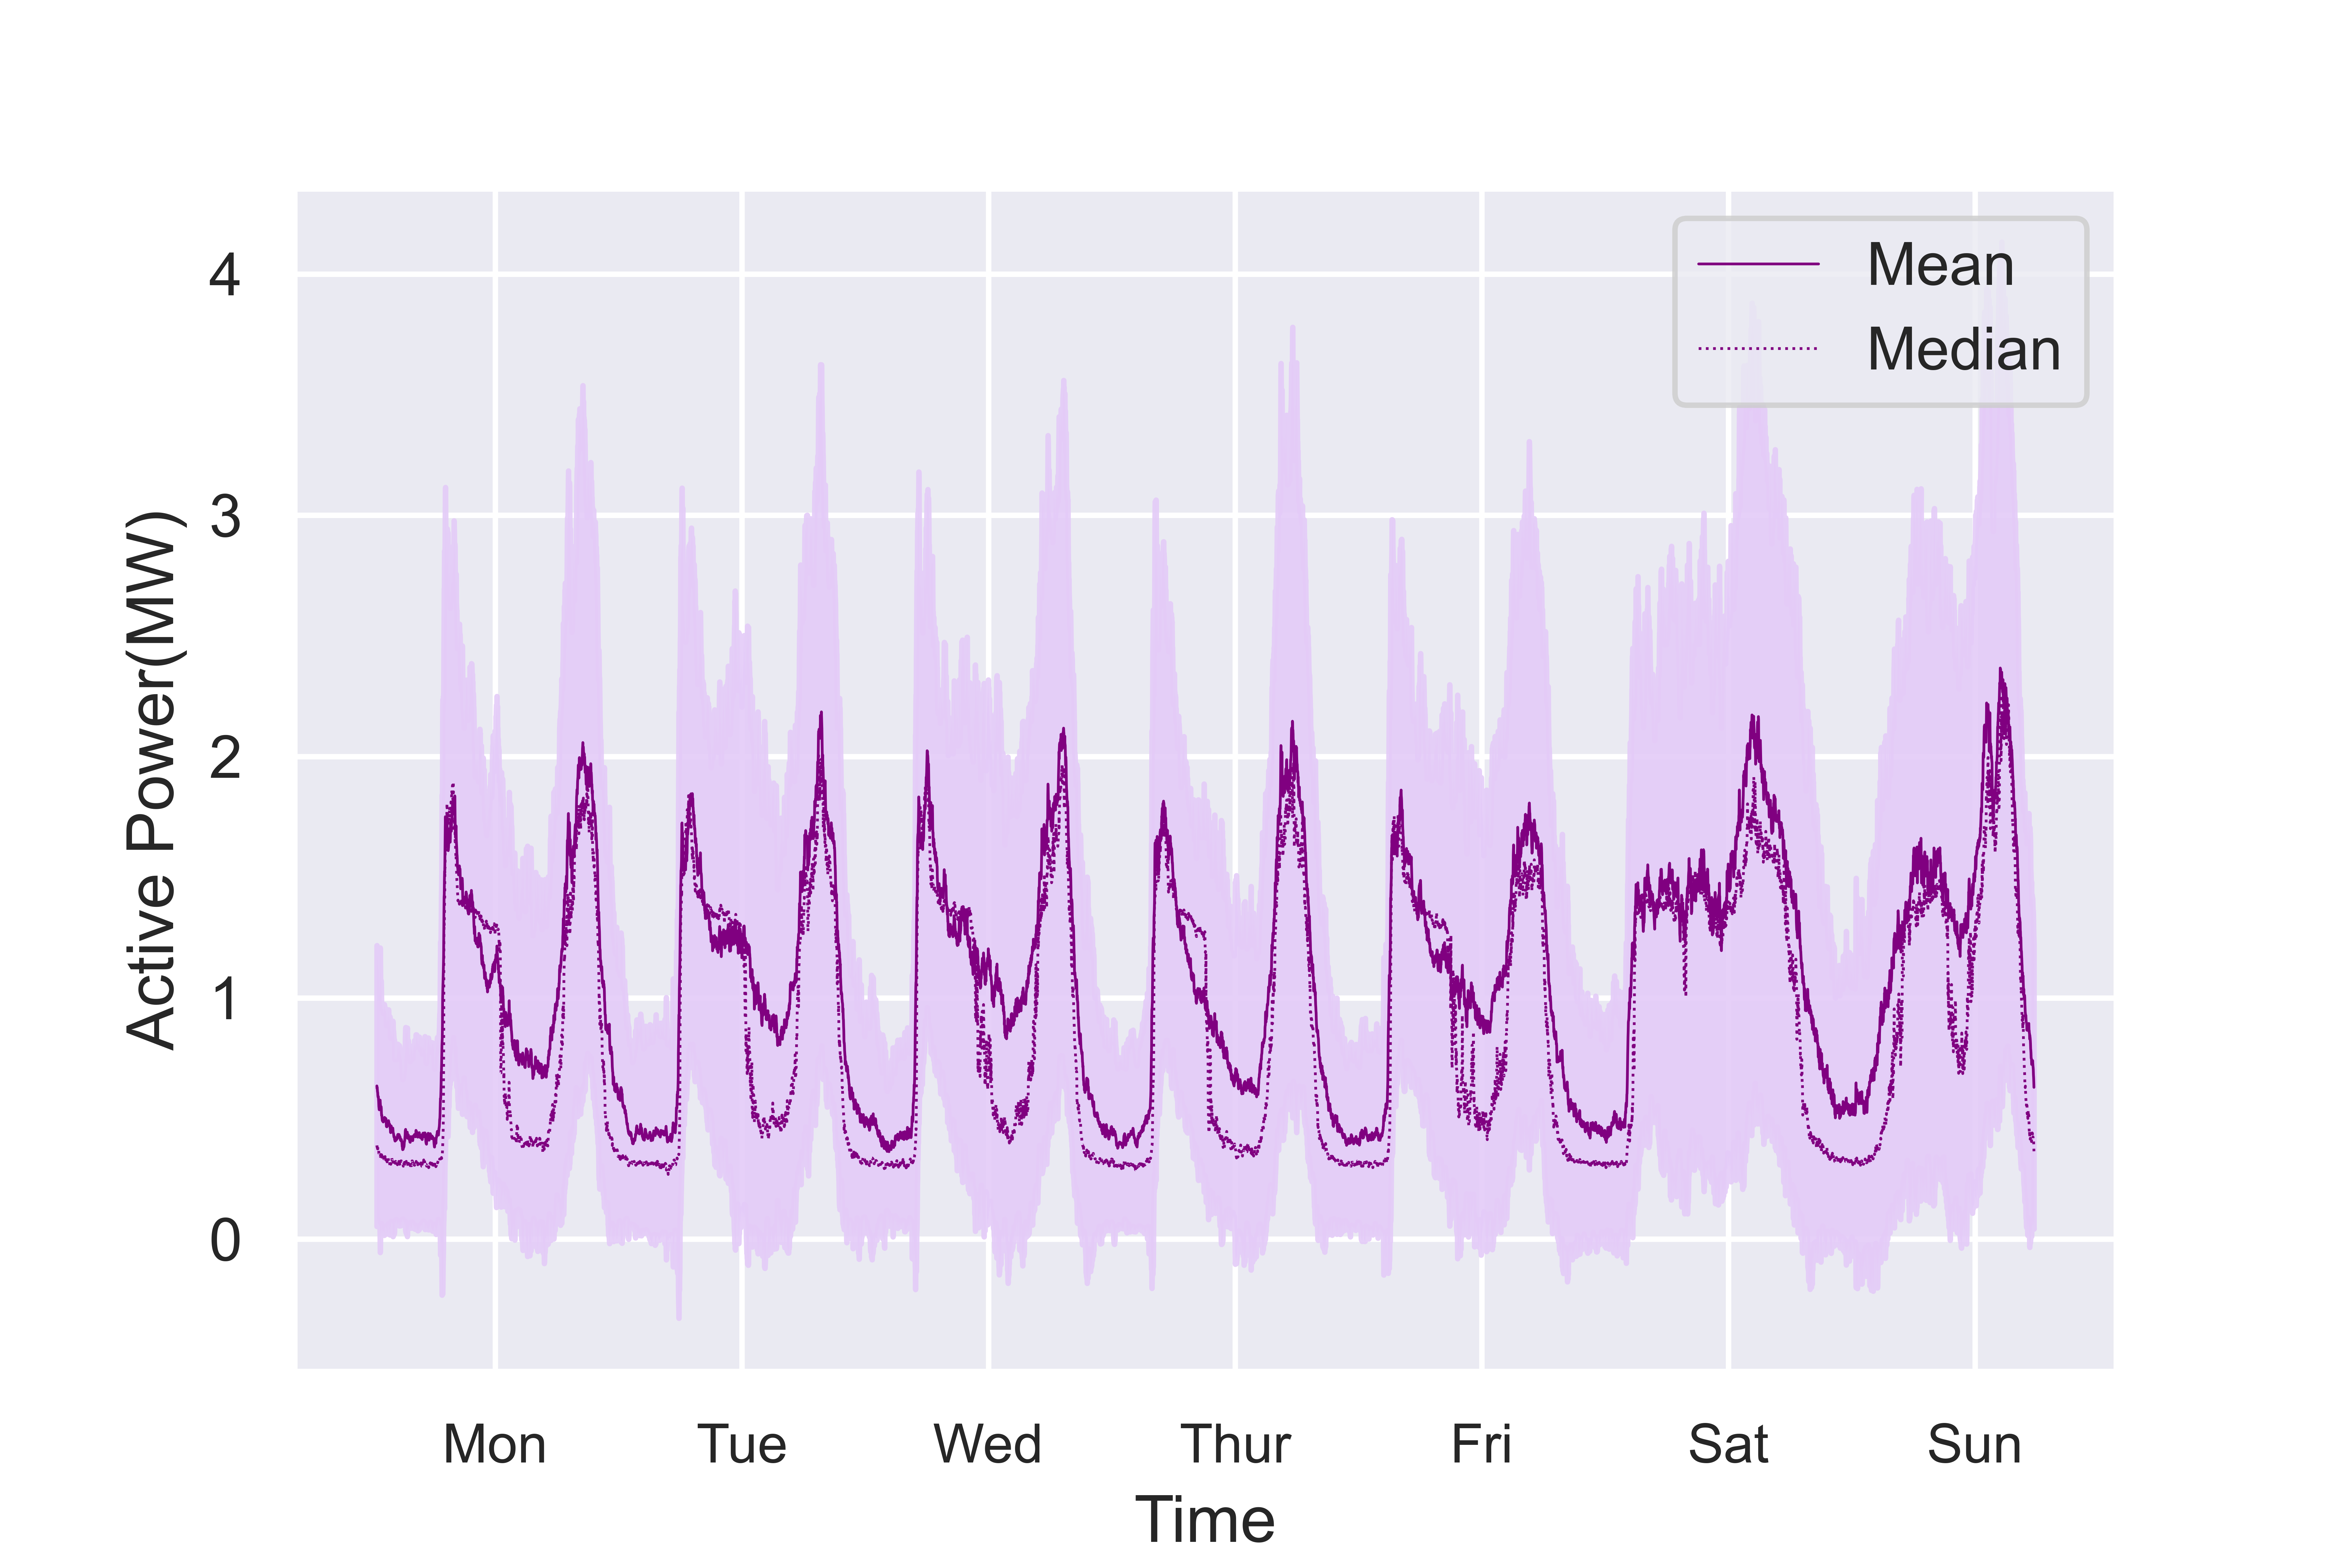
\includegraphics[width=\textwidth]{../Figures/uci.PNG}
% \end{figure}

\begin{figure}[H]
    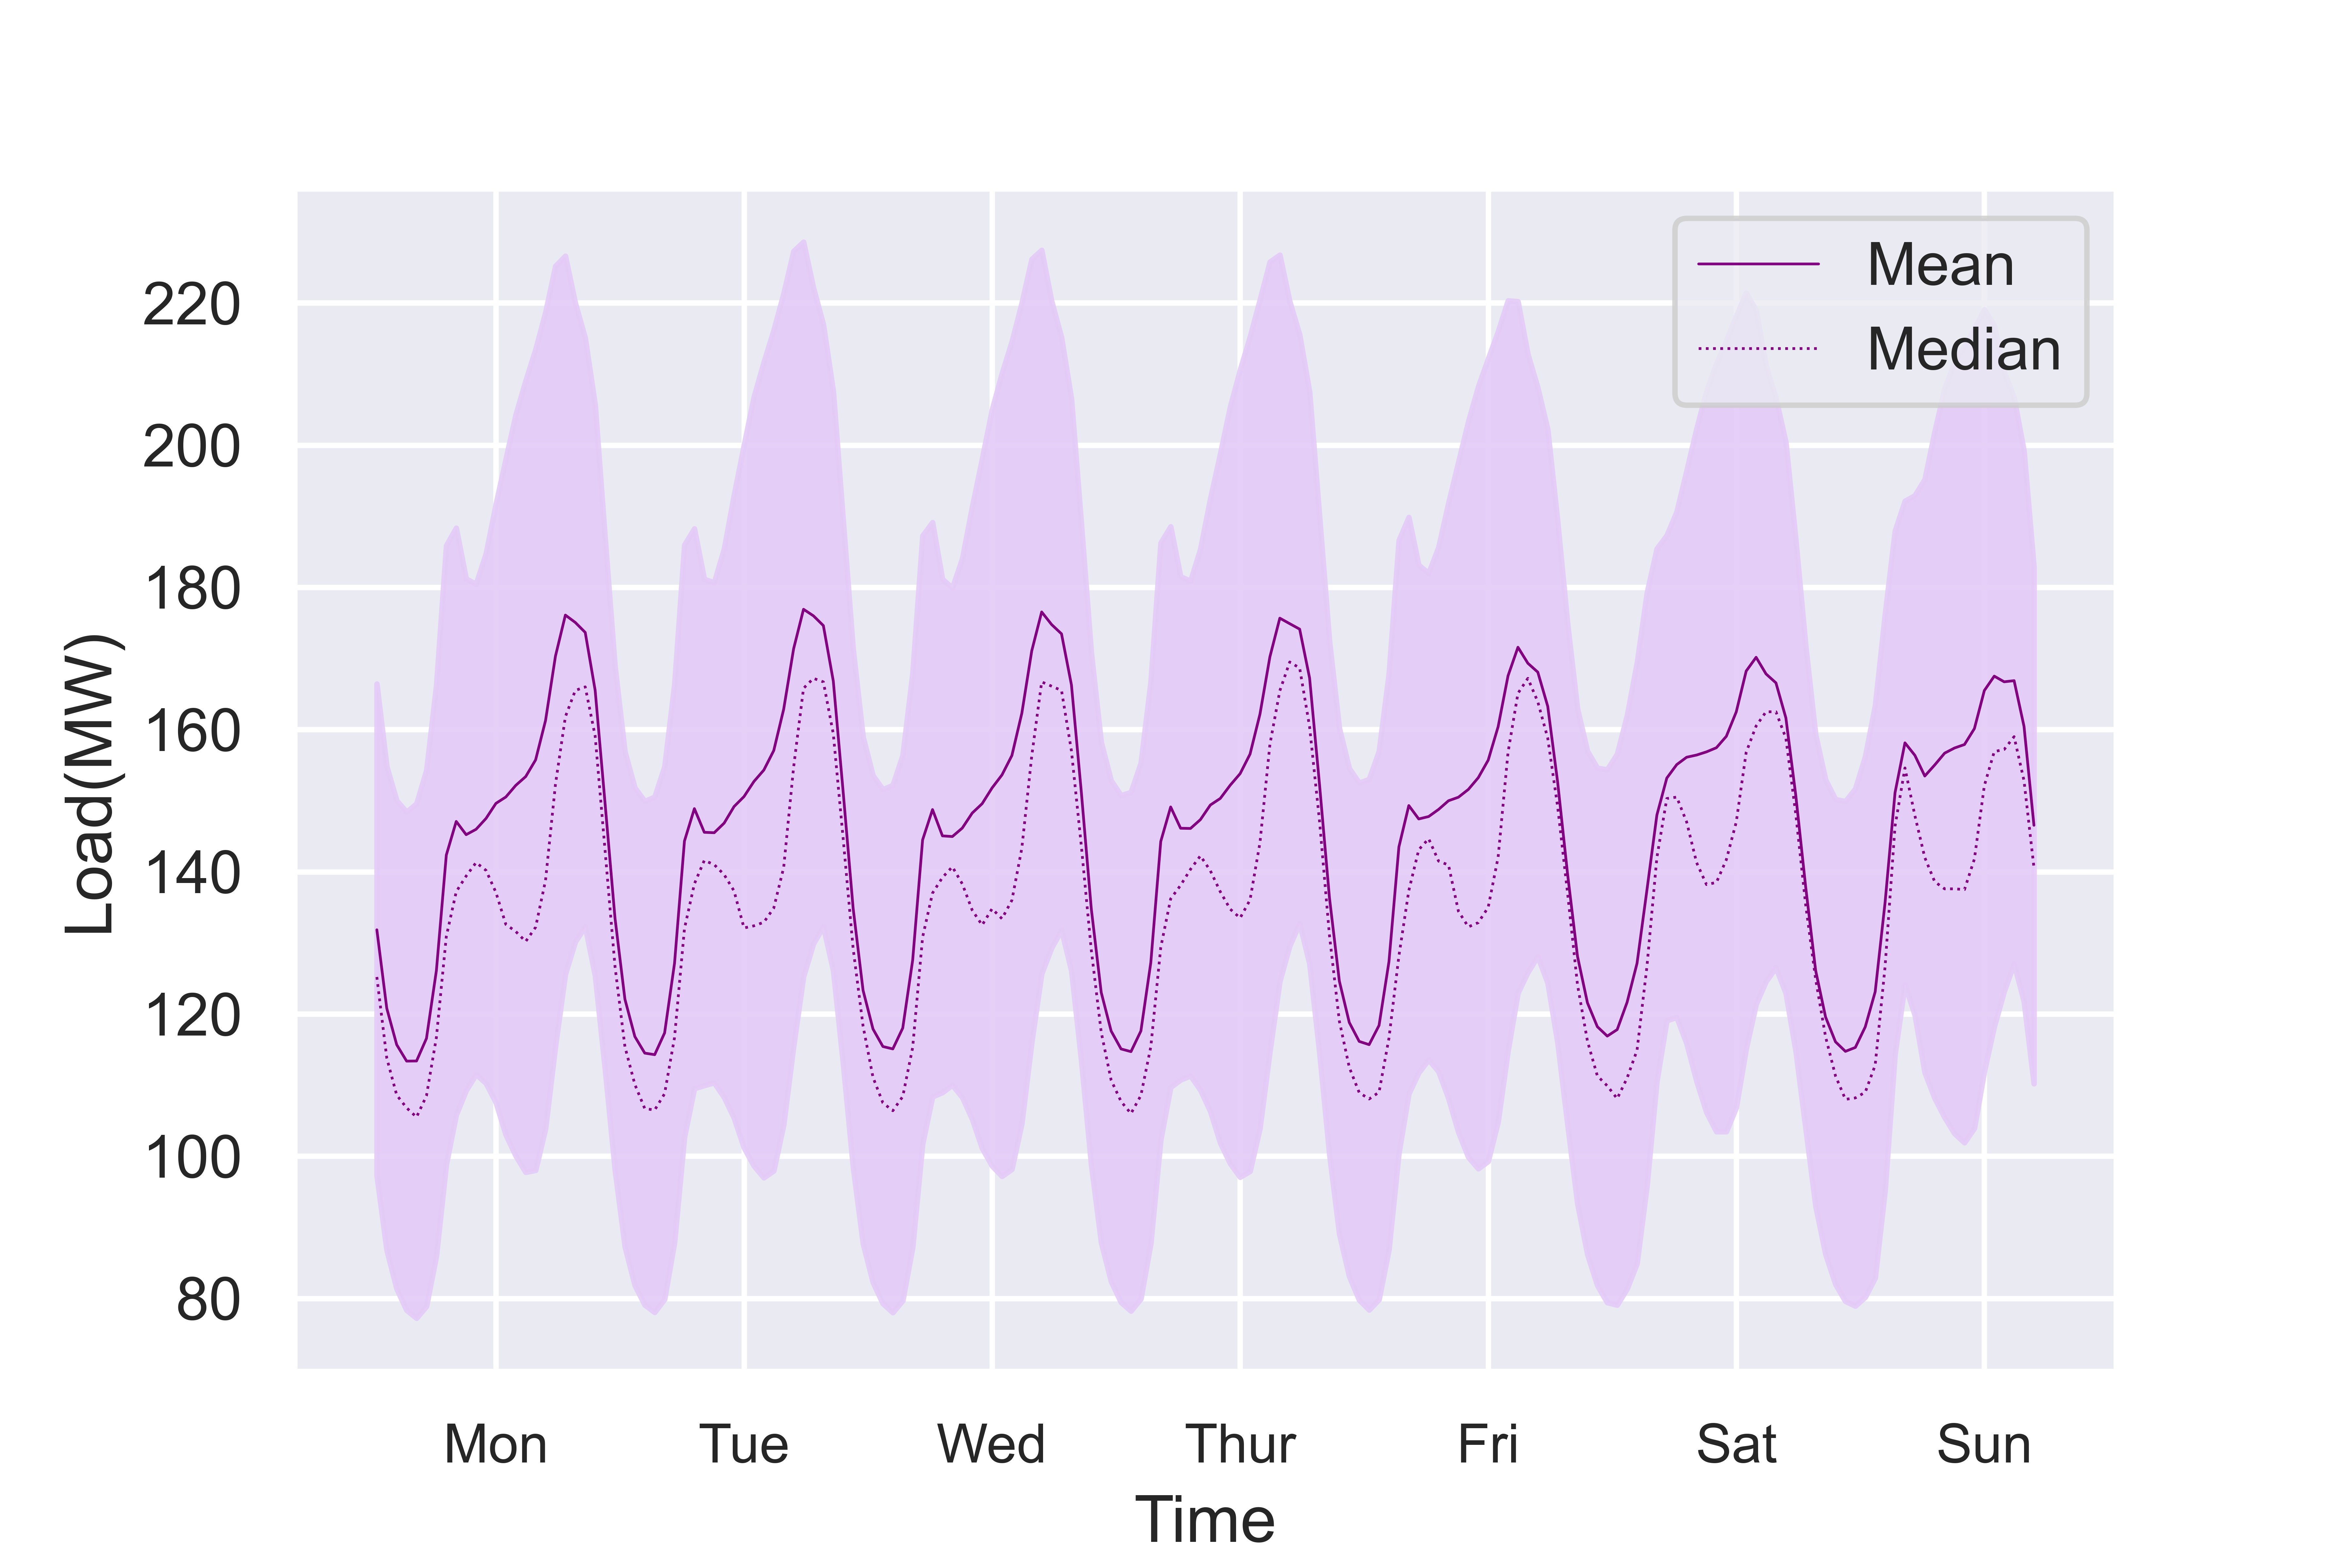
\includegraphics[width=\textwidth]{../Figures/gef2014.PNG}
    \caption{GEFCom2014 Electric Load}
    \label{fig:gefc2014}
\end{figure}

\section{Models and Evaluation}
In this experiment, TCN together with FNN, RNN, GRU, seq2seq models were adopted. And we use $MSE$,$RMSE$, $MAE$ and $R^2$ to evaluate models' performance. Besides, we also try to evaluate detection accuracy by using \textit{long-short prediction difference(LSPD)}. The definitions of these metrics are noted below.

$$RMSE = \sqrt[2]{\frac{1}{N}\sum_{i=0}^{N-1}\frac{1}{n_o}\sum_{t=0}^{n_o-1}(\hat{y_i}[t]-y_i[t])^2} $$
$$MAE = \frac{1}{N}\sum_{i=0}^{N-1}\frac{1}{n_o}\sum_{t=0}^{n_o-1}|\hat{y_i}[t]-y_i[t]|$$
$$R^2 = \frac{1}{N}\sum_{i=0}^{N-1}(1- \frac{RSS}{TSS})$$
$$RSS=\frac{1}{n_o}\sum_{t}^{n_o}(\hat{y_i}[t]-y_i[t])^2 \quad TSS= \frac{1}{n_o}\sum_{t}^{n_o}(y_i[t] - \overline{y}_i)^2 $$
$$MSE = \frac{1}{N}\sum_{i=0}^{N-1}\frac{1}{n_o}\sum_{t=0}^{n_o-1}(\hat{y_i}[t]-y_i[t])^2$$


\section{Programming Environment and Experiment Settings}
We adopted Keras framework to help us build such a experiment, related hardware and software dependencies as following table \ref{tab:dependencies}. 

\begin{table}[H]
\centering
\caption{Hardware and software dependencies}
\begin{tabular}{l l}
\toprule
\textbf{Item} & \textbf{Dependencies}  \\
\midrule
Cloud Computation Support & Supported by CityU Burgundy HPC\\
Python & Version 3.6.x  \\
TensorFlow& Version 2.1 \\
Keras& 2.3.1 \\
sacred& 0.7.5 \\
\bottomrule
\end{tabular}
\label{tab:dependencies}
\end{table}

\section{Numeric Results and Discussion}

\subsection{Models' performance comparison}
\begin{table}[H]
\centering
\caption{Models' Performance Comparison}
\begin{tabular}{l r r r r}
\toprule
\textbf{Model} & \textbf{MSE} & \textbf{MAE} & \textbf{$R^2$}& \textbf{RMSE}\\
\midrule
TCN & 772.69& 18.57& 0.86& 27.80\\
GRU\-Rec & 746.99& 19.64& 0.79& 27.33 \\
GRU\-MIMO& 423.54& 15.50& 0.82& 20.58 \\
Vanilla RNN& 2275.85& 30.47& 0.73& 47.71 \\
LSTM\-Rec & 697.94& 24.65& 0.76& 26.42 \\
LSTM\-MIMO & 378.31& 16.18& 0.87& 19.45 \\
FNN & 330.90& 10.53& \color{red}0.88& 18.19 \\
\bottomrule
\end{tabular}
\label{tab:models}
\end{table}

From table \ref{tab:models} we can find that FNN shows the best fit result amongst all the models we have adopted, with the $R^2 = 0.88$. Since TCN did not reach a good detection performance as other models did, so we did more sub-experiments on TCN, mainly on hyper-parameters modification and different datasets (not yet).

\begin{figure}[htbp]
\centering
\subfloat[fnn1]{
    \begin{minipage}[t]{0.5\textwidth}
    \centering
    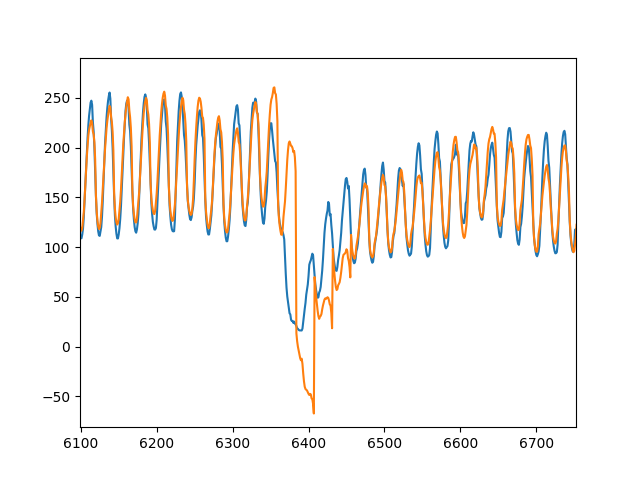
\includegraphics[width=6.5cm]{../Figures/fnn-1.png}
    \end{minipage}
}
\subfloat[fnn2]{
    \begin{minipage}[t]{0.5\textwidth}
    \centering
    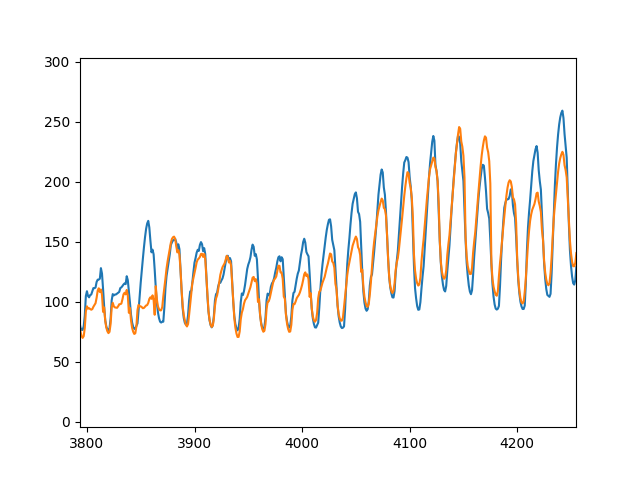
\includegraphics[width=6.5cm]{../Figures/fnn-2.png}
    \end{minipage}
}

\subfloat[fnn3]{
    \begin{minipage}[t]{0.5\textwidth}
    \centering
    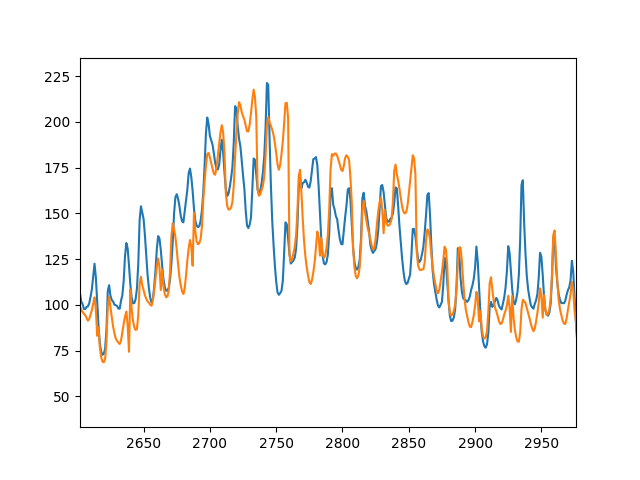
\includegraphics[width=6.5cm]{../Figures/fnn-3.png}
    \end{minipage}
    }
\subfloat[fnn4]{    
    \begin{minipage}[t]{0.5\textwidth}
    \centering
    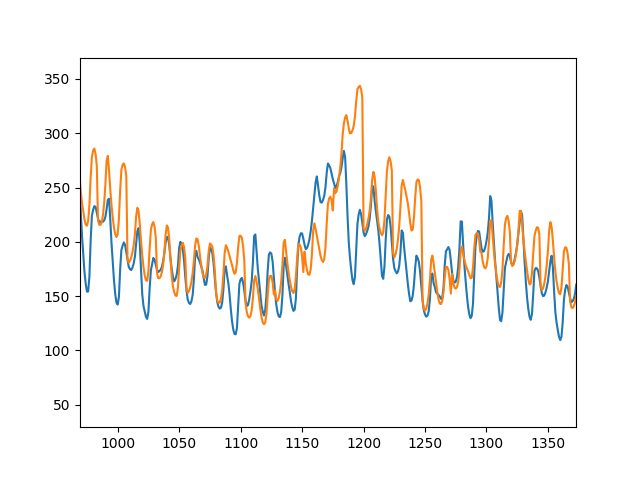
\includegraphics[width=6.5cm]{../Figures/fnn-4.png}
    \end{minipage}
}
\caption{Plots of FNN results} 
\label{FNN}%                         
\end{figure}

\begin{figure}[htbp]
\centering
\subfloat[tcn1]{
    \begin{minipage}[t]{0.48\textwidth}
    \centering
    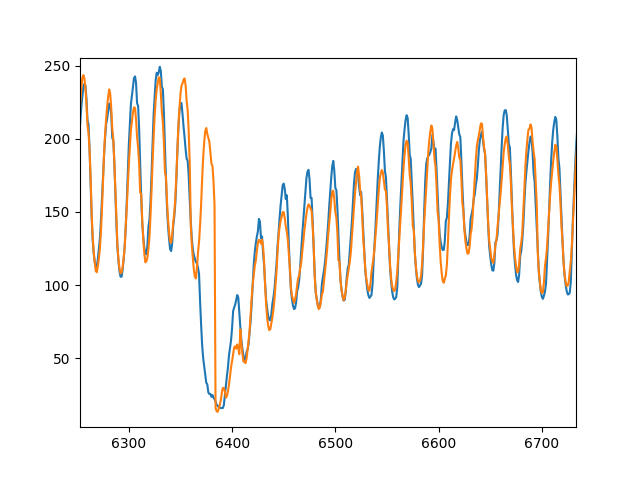
\includegraphics[width=6.5cm]{../Figures/tcn-1.png}
    \end{minipage}
}
\subfloat[tcn2]{
    \begin{minipage}[t]{0.48\textwidth}
    \centering
    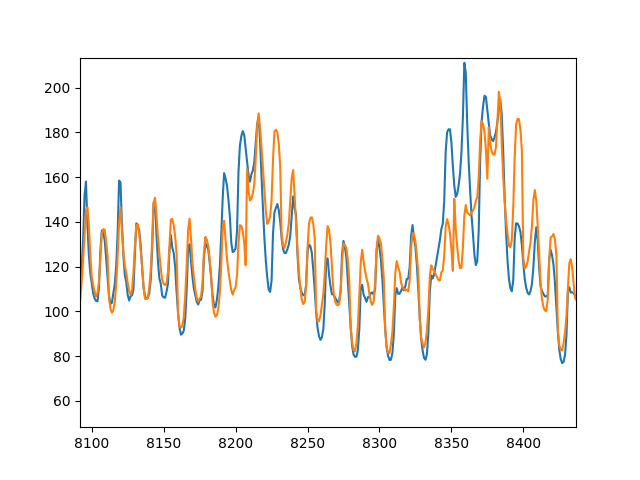
\includegraphics[width=6.5cm]{../Figures/tcn-2.png}
    \end{minipage}
}

\subfloat[tcn3]{
    \begin{minipage}[t]{0.48\textwidth}
    \centering
    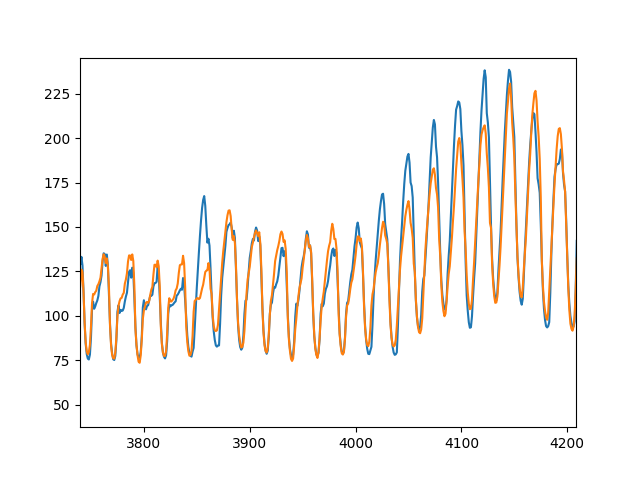
\includegraphics[width=6.5cm]{../Figures/tcn-3.png}
    \end{minipage}
    }
\subfloat[tcn4]{    
    \begin{minipage}[t]{0.48\textwidth}
    \centering
    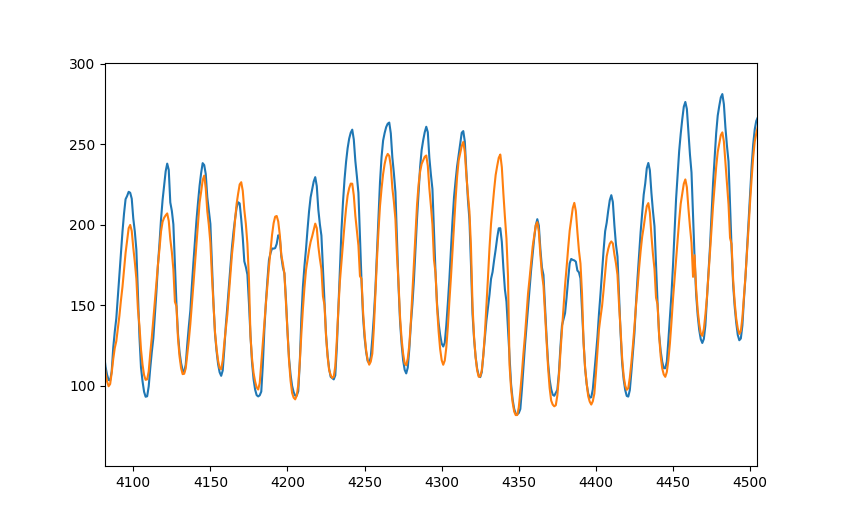
\includegraphics[width=6.5cm]{../Figures/tcn-4.png}
    \end{minipage}
}
\caption{Plots of TCN results} 
\label{TCN}%                         
\end{figure}

\begin{figure}[htbp]
\centering
\subfloat[gru-mimo1]{
    \begin{minipage}[t]{0.48\textwidth}
    \centering
    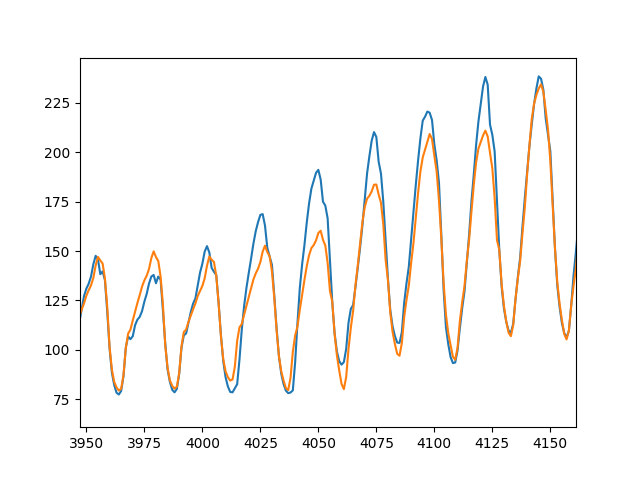
\includegraphics[width=6.5cm]{../Figures/gru-mimo-1.png}
    \end{minipage}
}
\subfloat[gru-mimo2]{
    \begin{minipage}[t]{0.48\textwidth}
    \centering
    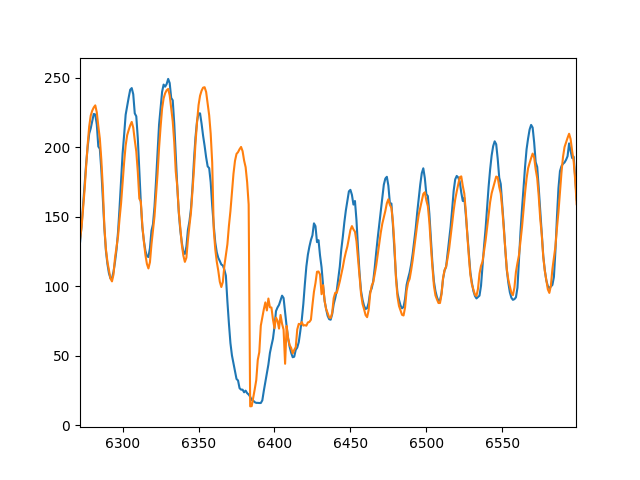
\includegraphics[width=6.5cm]{../Figures/gru-mimo-2.png}
    \end{minipage}
}

\subfloat[gru-mimo3]{
    \begin{minipage}[t]{0.48\textwidth}
    \centering
    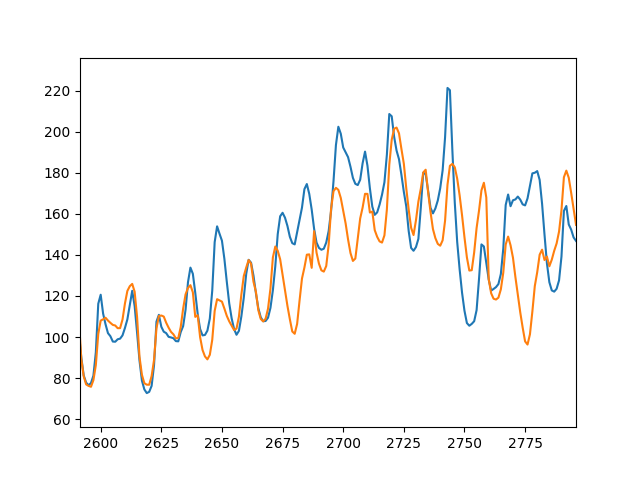
\includegraphics[width=6.5cm]{../Figures/gru-mimo-3.png}
    \end{minipage}
    }

\caption{Plots of GRU-MIMO results} 
\label{GRU-MIMO}%                         
\end{figure}

% \begin{figure}
%     \centering
%     \begin{subfigure}[b]{0.55\textwidth}
%         \centering
%         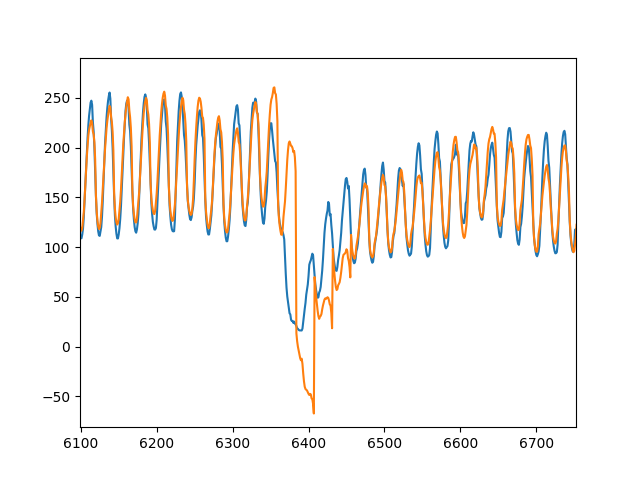
\includegraphics[width=\textwidth]{../Figures/fnn-1.png}
%         \caption{fnn1}
%         \label{fig:fnn1}
%     \end{subfigure}
%     \hfill
%     \begin{subfigure}[b]{0.55\textwidth}
%         \centering
%         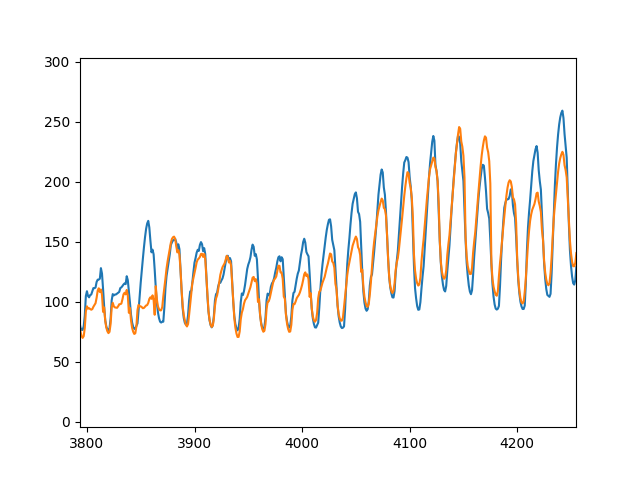
\includegraphics[width=\textwidth]{../Figures/fnn-2.png}
%         \caption{fnn2}
%         \label{fig:fnn2}
%     \end{subfigure}
%     \hfill
%     \begin{subfigure}[b]{0.55\textwidth}
%         \centering
%         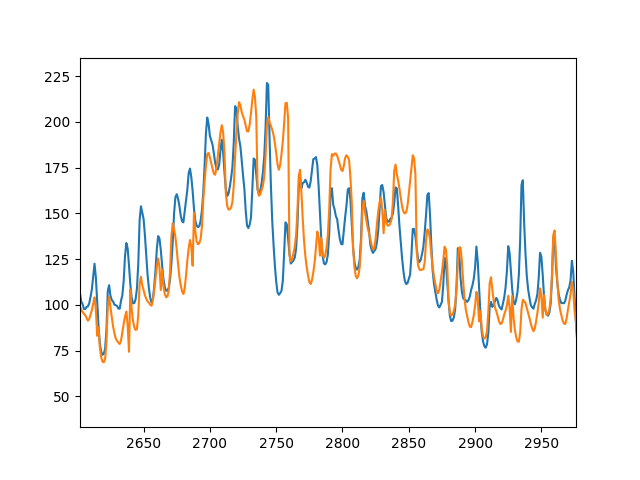
\includegraphics[width=\textwidth]{../Figures/fnn-3.png}
%         \caption{fnn3}
%         \label{fig:fnn3}
%     \end{subfigure}
%     \hfill
%     \begin{subfigure}[b]{0.55\textwidth}
%         \centering
%         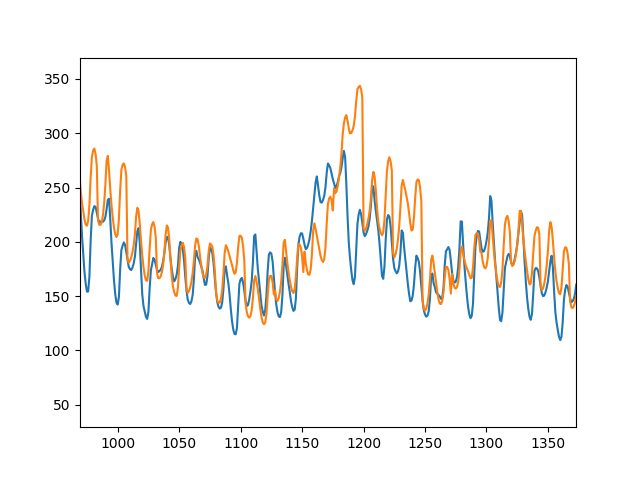
\includegraphics[width=\textwidth]{../Figures/fnn-4.png}
%         \caption{fnn4}
%         \label{fig:fnn4}
%     \end{subfigure}
%       \caption{FNN results in plot}
%       \label{fig:fnn}
% \end{figure}


% \begin{figure}
%     \centering
%     \begin{subfigure}[b]{0.55\textwidth}
%         \centering
%         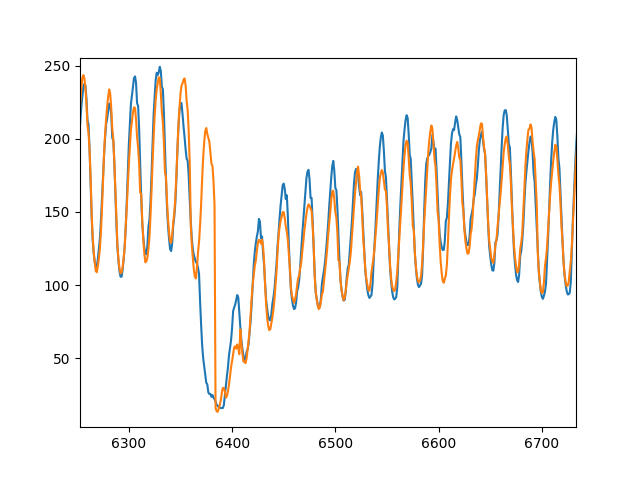
\includegraphics[width=\textwidth]{../Figures/tcn-1.png}
%         \caption{tcn1}
%         \label{fig:tcn1}
%     \end{subfigure}
%     \hfill
%     \begin{subfigure}[b]{0.55\textwidth}
%         \centering
%         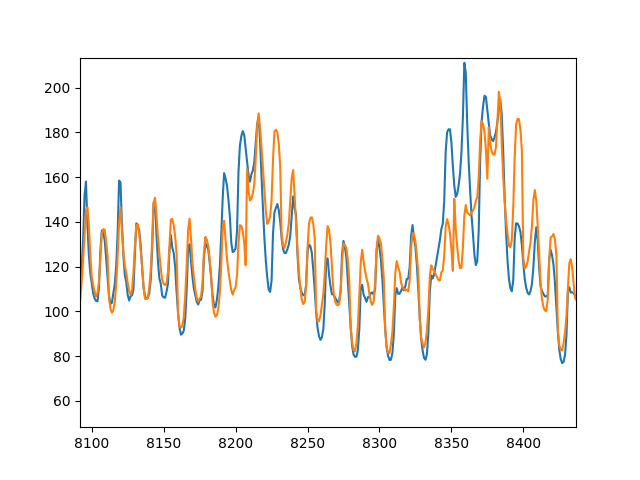
\includegraphics[width=\textwidth]{../Figures/tcn-2.png}
%         \caption{tcn2}
%         \label{fig:tcn2}
%     \end{subfigure}
%     \hfill
%     \begin{subfigure}[b]{0.55\textwidth}
%         \centering
%         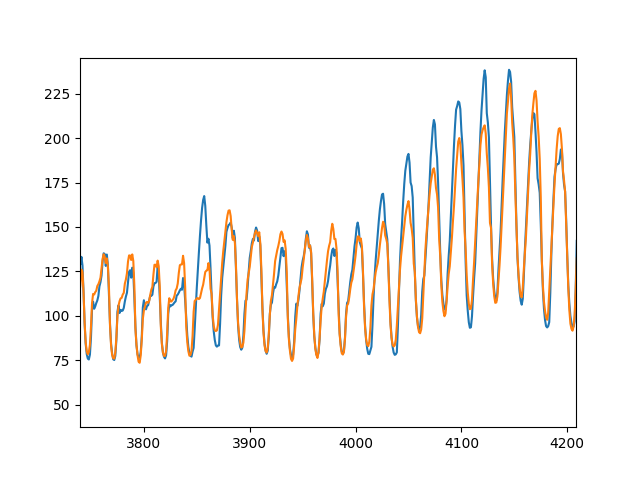
\includegraphics[width=\textwidth]{../Figures/tcn-3.png}
%         \caption{tcn3}
%         \label{fig:tcn3}
%     \end{subfigure}
%     \hfill
%     \begin{subfigure}[b]{0.55\textwidth}
%         \centering
%         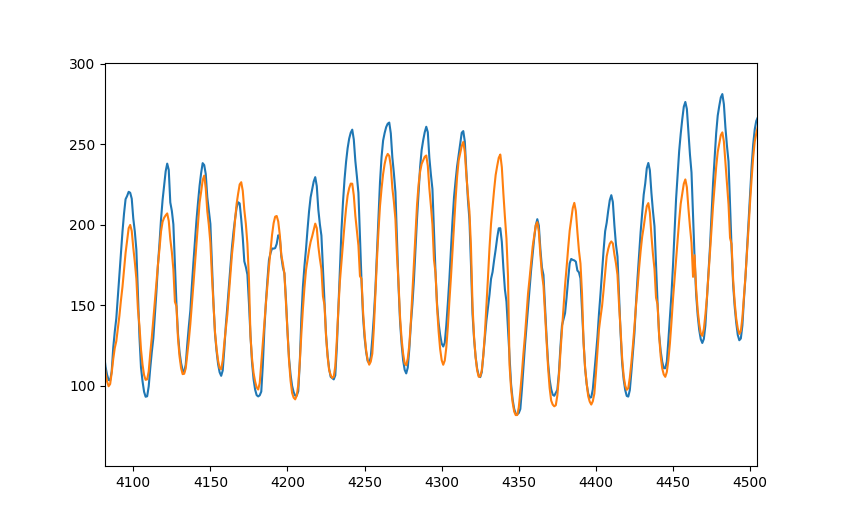
\includegraphics[width=\textwidth]{../Figures/tcn-4.png}
%         \caption{tcn4}
%         \label{fig:tcn4}
%     \end{subfigure}
%       \caption{TCN results in plot}
%       \label{fig:tcn}
% \end{figure}

% \begin{figure}
%     \centering
%     \begin{subfigure}[b]{0.55\textwidth}
%         \centering
%         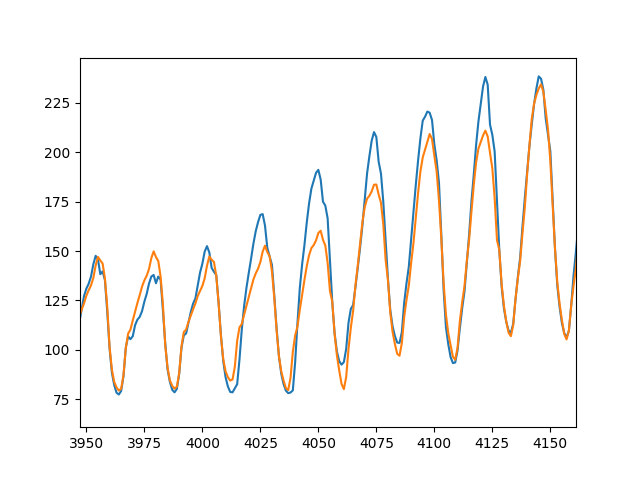
\includegraphics[width=\textwidth]{../Figures/gru-mimo-1.png}
%         \caption{gru-mimo1}
%         \label{fig:gru-mimo1}
%     \end{subfigure}
%     % \hfill
%     \begin{subfigure}[b]{0.55\textwidth}
%         \centering
%         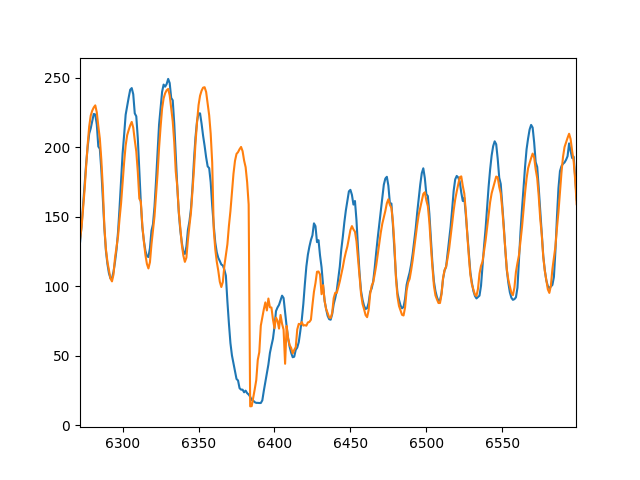
\includegraphics[width=\textwidth]{../Figures/gru-mimo-2.png}
%         \caption{gru-mimo2}
%         \label{fig:gru-mimo2}
%     \end{subfigure}
%     % \hfill
%     \begin{subfigure}[b]{0.55\textwidth}
%         \centering
%         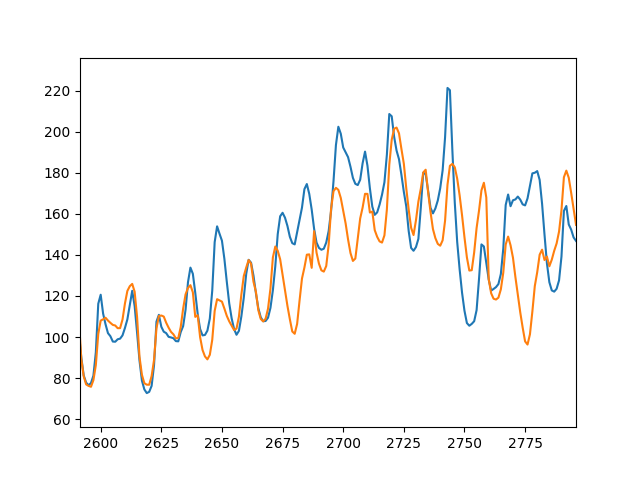
\includegraphics[width=\textwidth]{../Figures/gru-mimo-3.png}
%         \caption{gru-mimo3}
%         \label{fig:gru-mimo3}
%     \end{subfigure}
%       \caption{GRU-MIMO results in plot}
%       \label{fig:gru-mimo}
% \end{figure}


\subsection{TCN Improvement}
\begin{table}[H]
\centering
\caption{Hyper Parameters Comparison}
\begin{tabular}{l r r r r r r r r r r  r r r}
\toprule
\textbf{Test} & \textbf{Epochs} & \textbf{Input} & \textbf{Output}& \textbf{Lrate} & \textbf{L2-reg} & \textbf{OChannel} & \textbf{MSE} & \textbf{MAE} & \textbf{$R^2$}& \textbf{RMSE} \\
\midrule
Raw & 1& 96& 24& 0.001& 0.005& 32& 772.69& 18.57& 0.54& 27.80\\
T1 & \color{blue}100& 96& 24& 0.001& 0.005& 32& 280.32& 10.38& 0.84& 16.74 \\
T2 & \color{blue}30& 24& 24& 0.001& 0.005& 32& 315.89& 10.83& 0.82& 17.77 \\
T3 & 30& \color{blue}48& 24& 0.001& 0.005& 32& 300.18& 10.58& 0.83& 17.33 \\
T4 & 30& \color{blue}96& 24& 0.001& 0.005& 32& 280.32& 10.38& 0.84& 16.74 \\
T5 & 30& \color{blue}168& 24& 0.001& 0.005& 32& 300.18& 10.58& 0.83& 17.33 \\
T6 & 30& \color{blue}336& 24& 0.001& 0.005& 32& 259.50& 9.91& 0.84& 16.11 \\ %14
T7 & 30& 336& \color{blue}48& 0.001& 0.005& 32& 370.97& 11.80& 0.76& 19.26 \\
T8 & 30& 168& 24& \color{blue}0.01& 0.005& 32& 265.36& 10.03& 0.84& 16.29 \\
T9 & 30& 168& 24& 0.001& \color{blue}0.001& 32& 256.22& 9.81& 0.86& 16.01 \\
T10 & 30& 168& 24& 0.001& \color{blue}0.01& 32& 266.83& 9.81& 0.84& 16.34 \\
T11 & 30& 168& 24& 0.001& 0.01& \color{blue}16& 254.09& 9.61& \color{red}0.864& 15.94 \\
\bottomrule
\end{tabular}
\label{tab:hyper}
\end{table}

As table \ref{tab:hyper} showed, we try to change input length and output length , which are how many hours will be used as a sliding window's input and output, to make the model more sensible, and according to test metrics, we found that TCN will give the best performance when we try to use 7 days (168 hours)' electricity load to predict one day(24 hours)'s electricity load, we got $R^2 \geq 0.85$.

As for Epochs, which means the number of passes of the entire training dataset the deep learning algorithm has completed, significantly influenced TCN's training, and 30 epochs will give the most economical training results. We guess this is because TCN needs more passes to fit a good state, for it lacks some mechanism like LSTM's recurrent units.

Learning rate, L2-regulation, and the number of out channels were also influenced, but they mainly contributed to improving computation speed.

% \newpage
\section{Further Discussion with Dataset Sensitivity of TCN and LSTM }
From the previous experiment result, the TCN model present a good performance with whole Gefcom2014 dataset, but it’s not the most outstanding one. Then here are some assumptions coming up: \\
1. Is the TCN would perform better in a high variance dataset than a low variance dataset, in other word, have a better performance on anomaly detection; \\
2. How much the size of dataset would influence the TCN fitted result. 
\subsection{Experiment on different variance data}
In order to find specific effects on different variance of data with TCN, we create four datasets derived from original Gefcom2014 data as object data, each data has different variance. The plots of the four datasets are below:

\begin{figure}[htbp]
\centering
\subfloat[data1]{
    \begin{minipage}[t]{0.48\textwidth}
    \centering
    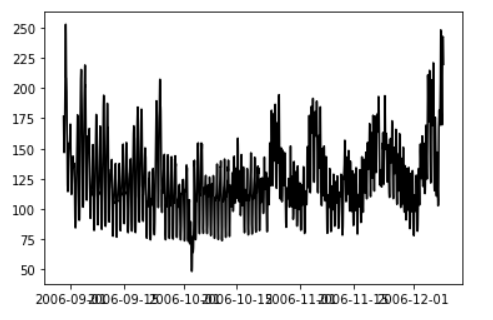
\includegraphics[width=6.5cm]{../Figures/data1.PNG}
    \end{minipage}
}
\subfloat[data2]{
    \begin{minipage}[t]{0.48\textwidth}
    \centering
    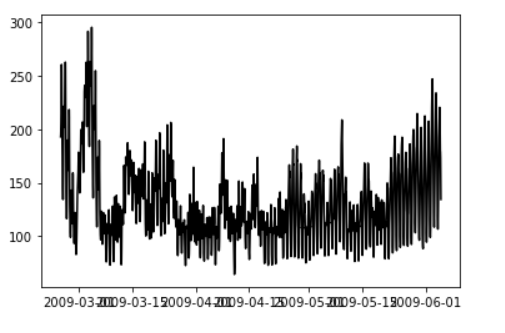
\includegraphics[width=6.5cm]{../Figures/data2.PNG}
    \end{minipage}
}

\subfloat[data3]{
    \begin{minipage}[t]{0.48\textwidth}
    \centering
    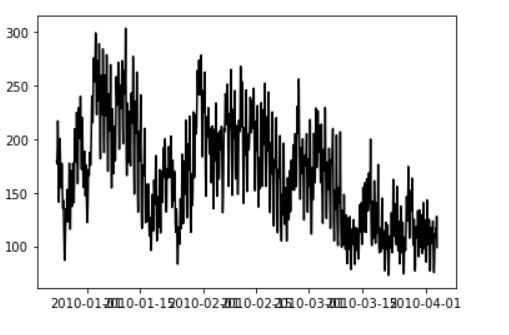
\includegraphics[width=6.5cm]{../Figures/data3.PNG}
    \end{minipage}
    }
\subfloat[data4]{    
    \begin{minipage}[t]{0.48\textwidth}
    \centering
    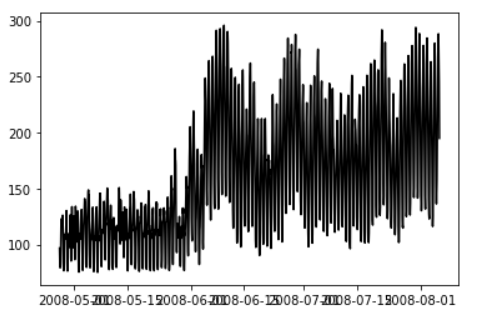
\includegraphics[width=6.5cm]{../Figures/data4.PNG}
    \end{minipage}
}
\caption{Plots of datasets} 
\label{Plots of datasets}%                         
\end{figure}

By applying TCN on datas, we get experiment results as below, and we use $R^2$ as measurement.
\begin{table}[H]
\centering
\caption{TCN Performance Comparison 1}
\begin{tabular}{l r r r r}
\toprule
\textbf{data}  & \textbf{data variance}& \textbf{$R^2$} & \textbf{epoch}& \textbf{stable epoch}\\
\midrule
data1 & 928.38 & 0.7201& 150& 110\\
data2 & 1380.28 & 0.7586& 150& 110 \\
data3 & 2263.21 & 0.9246& 150& 10 \\
data4 & 3200.74 & 0.7805& 150& 70 \\
\bottomrule
\end{tabular}
\label{tab:TCN}
\end{table}

In the table the 'stable epoch' means the amount of epochs the model needed to iterate and attain a stable $R^2$ value. From the results we find that with high variance data, TCN do perform better on $R^2$, which represent that TCN model is more sensitive to detect anomaly in time series data. However, for data3, the variance of it is not greater than data4, while the corresponding $R^2$ is higher. By comparing the data shape above, we can find that data4 is more likely a data merged by two stable datasets with a sharp connection between them, while data3 is a real fluctuated data. \\
And as LSTM also performs well with original data in previous experiment, we try to apply it on the four datasets as comparison. In order to make comparison the more convincing, most of the hyper-parameters in two models are stay the same. The results are shown below:
\begin{table}[H]
\centering
\caption{LSTM Performance Comparison 1}
\begin{tabular}{l r r r r}
\toprule
\textbf{data}  & \textbf{data variance}& \textbf{$R^2$} & \textbf{epoch}& \textbf{stable epoch}\\
\midrule
data1 & 928.38 & 0.7161 & 50& 30\\
data2 & 1380.28 & 0.7637 & 50& 30 \\
data3 & 2263.21 & 0.8385 & 50& 30 \\
data4 & 3200.74 & 0.7761 & 50& 30 \\
\bottomrule
\end{tabular}
\label{tab:LSTM}
\end{table}
The results show that LSTM also performs better in high variance data, and the $R^2$ in data3 is also greater than data4. but the $R^2$ improvement from low variance data to high variance data is not as much as TCN. The difference may because that in TCN, convolutional layer used to extract features, so that in fluctuated dataset, it would easier to extract useful features and improve the model performance, while in flatter dataset, it's advantage can not be applied and can hardly outperform other NN algorithms.
\subsection{Experiment on different size data}
In order to find specific effects on different size of data with TCN, we create four datasets derived from original Gefcom2014 data as training data, each data has different data size. The plots of the four datasets are below:
\begin{figure}[H]
\centering
\subfloat[data5]{
    \begin{minipage}[t]{0.48\textwidth}
    \centering
    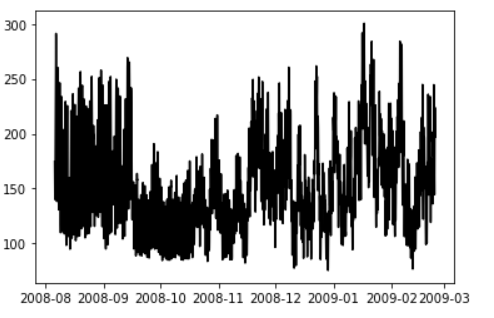
\includegraphics[width=6.5cm]{../Figures/data5.PNG}
    \end{minipage}
}
\subfloat[data6]{
    \begin{minipage}[t]{0.48\textwidth}
    \centering
    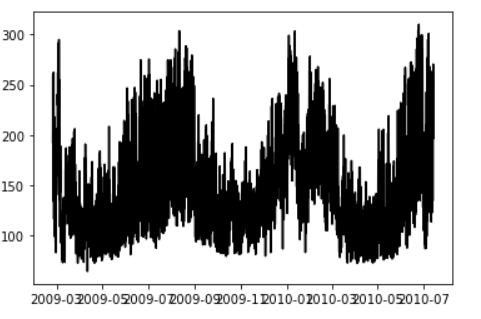
\includegraphics[width=6.5cm]{../Figures/data6.PNG}
    \end{minipage}
}

\subfloat[data7]{
    \begin{minipage}[t]{0.48\textwidth}
    \centering
    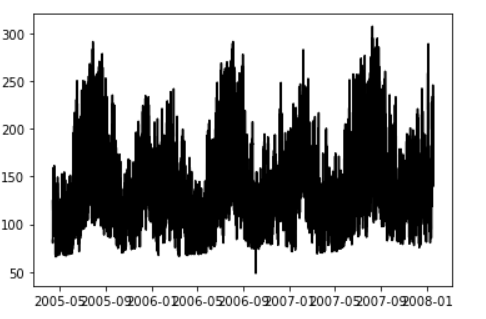
\includegraphics[width=6.5cm]{../Figures/data7.PNG}
    \end{minipage}
    }
\subfloat[data8]{    
    \begin{minipage}[t]{0.48\textwidth}
    \centering
    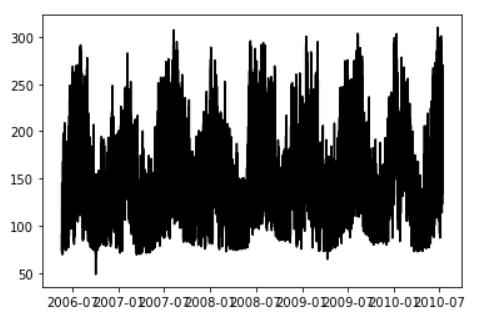
\includegraphics[width=6.5cm]{../Figures/data8.PNG}
    \end{minipage}
}
\caption{Plots of datasets 2} 
\label{Plots of datasets 2}%                         
\end{figure}
By applying TCN on datasets, we get experiment results as below:
\begin{table}[H]
\centering
\caption{TCN Performance Comparison 2}
\begin{tabular}{l r r r r}
\toprule
\textbf{data}  & \textbf{data size}& \textbf{$R^2$} & \textbf{epoch}& \textbf{stable epoch}\\
\midrule
data5 & 4848 & 0.7525 & 150& 70\\
data6 & 12120 & 0.8587 & 150& 30 \\
data7 & 24240 & 0.8591 & 150& 10 \\
data8 & 36360 & 0.8607 & 150& 10 \\
original data & 60600 & 0.8641& 150& 10 \\
\bottomrule
\end{tabular}
\label{tab:TCN2}
\end{table}
For long-term dataset, TCN would easily get a good fitted result with only 10 epochs training, while for short-term dataset, TCN perform worse and need more than 70 epochs training to provide a relatively good result.\\
And we also apply the same datas into LSTM model, here is table of LSTM training results:
\begin{table}[H]
\centering
\caption{LSTM Performance Comparison 2}
\begin{tabular}{l r r r r}
\toprule
\textbf{data}  & \textbf{data size}& \textbf{$R^2$} & \textbf{epoch}& \textbf{stable epoch}\\
\midrule
data5 & 4848 & 0.8149 & 50& 30\\
data6 & 12120 & 0.8441 & 50& 20 \\
data7 & 24240 & 0.8656 & 50& 10 \\
data8 & 36360 & 0.8674 & 50& 10 \\
original data & 60600 & 0.8763& 50& 10 \\
\bottomrule
\end{tabular}
\label{tab:LSTM2}
\end{table}
For the $R^2$ of long-term data and short-term data, LSTM also get a lower improvement compared to TCN, which means that TCN is more sensitive to the data size. However, when faced a small dataset, LSTM need fewer epochs to attain the relative optimal point than TCN, which indicates that LSTM would be more efficient in time series data training while applying on small sample. One of the reasons is that TCN model have convolutional layers with more parameters need to be iterated. When LSTM is processing, only one hidden state need to be concentrate on and every state get one single input, while for TCN, it request a long enough sequence to keep the history state, which require a bigger memory. However, since the same filter is used in each layer, convolutions can be done in parallel, so that TCN would be more efficient on huge dataset instead of small dataset.

\section{Discussion with kernel adjustment and improved performance}
In the previous discussion, we find TCN perform worse for short-term dataset than long-term dataset, and will take more training epochs to provide a relatively good result, which indicates that TCN is more sensitive to the data size and also time-consuming although it allows for parallel computation of outputs. In order to improve this problem, we did some adjustment to our convolutional kernel to have a bigger receptive field. The architecture of TCN employs dilated convolutions that enable an exponentially large receptive field. Using larger dilation enables an output at the top level to represent a wider range of inputs, there are two ways to increase the receptive field of TCN: choosing lager filter sizes k and increasing the dilation factor d. After doing some adjustment to TCN's convolutional kernel, the updated result is shown below:

\begin{table}[H]
\centering
\caption{Models' Performance with TCN's Kernel Adjustment}
\begin{tabular}{l r r r r}
\toprule
\textbf{Model} & \textbf{MSE} & \textbf{MAE} & \textbf{$R^2$}& \textbf{RMSE}\\
\midrule
TCN & 772.69& 18.57& 0.86& 27.80\\
TCN(kernel adjustment) & 284.35 & 10.02 & \color{red}0.91& 16.88\\
GRU\-Rec & 746.99& 19.64& 0.79& 27.33 \\
GRU\-MIMO& 423.54& 15.50& 0.82& 20.58 \\
Vanilla RNN& 2275.85& 30.47& 0.73& 47.71 \\
LSTM\-Rec & 697.94& 24.65& 0.76& 26.42 \\
LSTM\-MIMO & 378.31& 16.18& 0.87& 19.45 \\
FNN & 330.90& 10.53& 0.88& 18.19 \\
\bottomrule
\end{tabular}
\label{tab:kernal}
\end{table}

The result shows that TCN can achieve the best performance among all models in this electronic grid load issues. TCN model has a flexible receptive field size, which can be adjusted according to different application situation and tasks. which afford better control of the model’s memory size, and are easy to adapt to different domains. The improved TCN model is less sensitive to data size, speeds up iteration and improves predicting performance. Our result also shows that TCN can be served as a convenient but powerful starting point when dealing with sequential data. 

\section{Speed Up with Attention Mechanism}
Since TCN needs a huge computatial resources to fit a good model state, although we could enlarge sensitive field to decrease the complity but from other side, the structure of deep network should be more effective. From the original transform of sequence modeling, researchers try to imporve performance on this aspect by two methods, the one is using convolution layers, the other is using attention mechanism. We imported encoding and decoding capsule to warp the TCN moduels, and modify the core network structure as following. 

The performance of the new structure list the below table.
\begin{table}[H]
\centering
\caption{Speed of TCN and Attention Capsuled TCN}
\begin{tabular}{l c c}
\toprule
\textbf{Model} & \textbf{$R^2$}& \textbf{Training Time(Second)}\\
\midrule
Raw TCN &0.86& 278\\
Attention Capsuled TCN &0.69 & 163\\
\bottomrule
\end{tabular}
\label{tab:attentionTCN}
\end{table}